\documentclass[12pt]{article}
\usepackage{amsmath,amssymb,latexsym}
\usepackage{graphicx,psfrag,epsf}
\usepackage{enumerate}
\usepackage{natbib}
\usepackage{wrapfig}

\newcommand{\blind}{0}

\addtolength{\oddsidemargin}{-.75in}%
\addtolength{\evensidemargin}{-.75in}%
\addtolength{\textwidth}{1.5in}%
\addtolength{\textheight}{1.3in}%
\addtolength{\topmargin}{-.8in}%
\pagenumbering{gobble}

\begin{document}
\pagenumbering{arabic}

%\bibliographystyle{natbib}

\def\spacingset#1{\renewcommand{\baselinestretch}%
{#1}\small\normalsize} \spacingset{1}


%%%%%%%%%%%%%%%%%%%%%%%%%%%%%%%%%%%%%%%%%%%%%%%%%%%%%%%%%%%%%%%%%%%%%%%%%%%%%%

\if0\blind
{
  \title{\bf It is Impossible to Achieve a Spring-magnetic Perpetual Motion Machine }
  \author{Stanley Zheng}
  \maketitle
} \fi

\if1\blind
{
  \bigskip
  \bigskip
  \bigskip
  \begin{center}
    {\LARGE\bf Title}
\end{center}
  \medskip
} \fi

\bigskip
\begin{abstract}
Perpetual motion machines are hypothetical mechanical devices that can operate indefinitely without an external energy or energy input and can continuously do work while having only one heat source. Throughout history, people have been enthusiastic about developing various types of perpetual motion machines. Although science has proven that a certain class of perpetual motion machines is entirely impossible, many individuals continue to attempt to construct such devices. This article aims to demonstrate, theoretically and through quantitative calculations, that a perpetual motion machine composed of permanent magnets and springs is not achievable.
\end{abstract}


\spacingset{1.45}
\section{Introduction}
\label{sec:intro}

Perpetual motion machines are typically classified into two categories: the first kind and the second kind. The first kind of perpetual motion machine is one that can perform work without the need for an external energy source. Over the centuries, numerous individuals have attempted to design or construct such machines in a quest to find a way to produce infinite energy. However, the first law of thermodynamics theoretically refutes this idea. After it was proven that the first kind of perpetual motion machine is impossible to create, the exploration of perpetual motion did not cease. Instead of pursuing the creation of something from nothing, researchers aimed to develop machines with no losses. These machines would have a single heat source from which all absorbed heat could be entirely converted into work without causing any other changes. Such machines are referred to as the second kind of perpetual motion machine. Nevertheless, the second law of thermodynamics also theoretically demonstrates the impossibility of constructing macroscopic second-kind perpetual motion machines. Despite numerous theoretical proofs, there are still individuals who entertain the idea of creating perpetual motion machines. As the Figure 1 shown below, there is a conceptual diagram of a perpetual motion machine. At the center of this machine is a large permanent magnet, surrounded by slender rods. One end of each rod is fixed to a rotating axle, while the other end is attached to a spring, with a small permanent magnet fixed to the opposite end of the spring. When the small magnet aligns with the large magnet, the opposite magnetic polarities generate a repulsive force that propels the small magnet outward. This causes an increase in the lever arm for gravitational force, where the inward torque from gravity is greater than the outward torque, resulting in clockwise rotation of the entire axle. Once the small magnet moves away from the region with the strongest influence of the large magnet, the spring brings it back to its original position. This action shortens the lever arm for the gravitational force, which forms an inward torque. Consequently, the entire device can perpetually perform work.

\begin{figure}[h]
\hspace*{1.5cm}
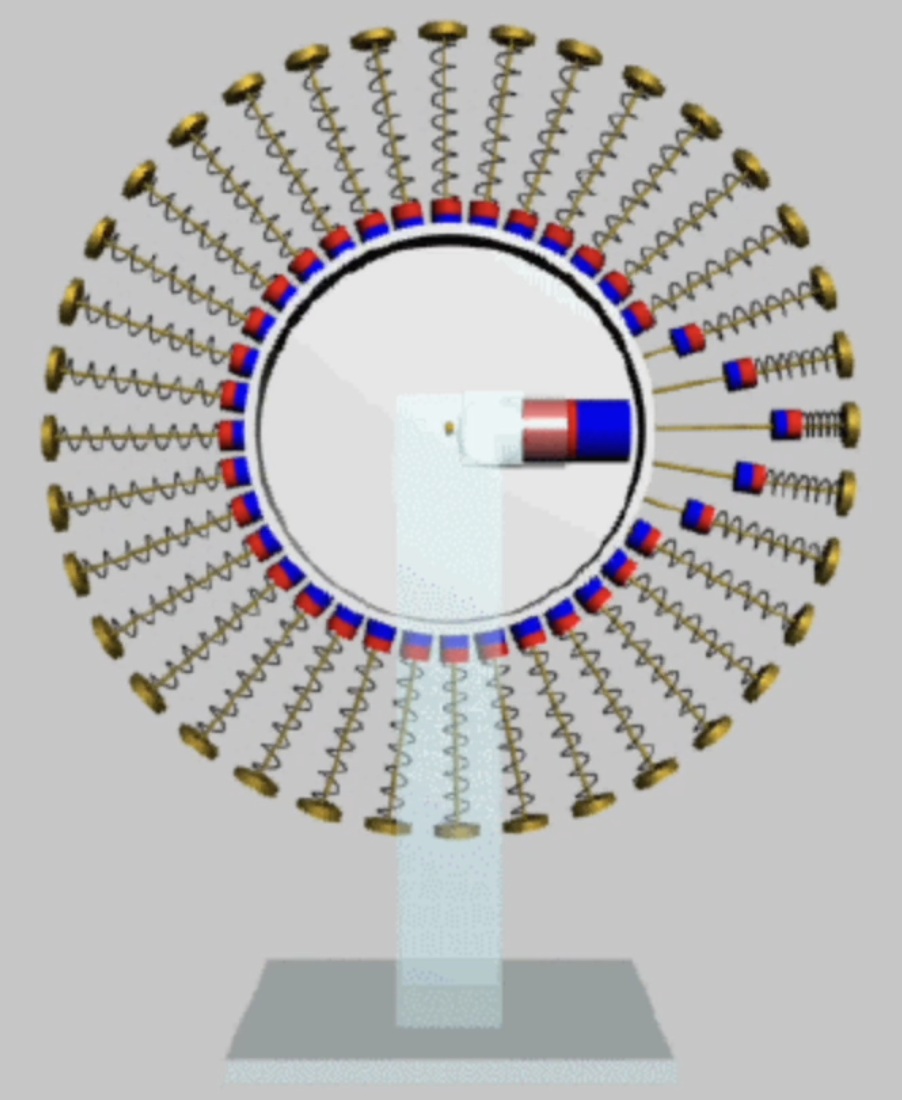
\includegraphics[width=0.2\linewidth]{1.png}
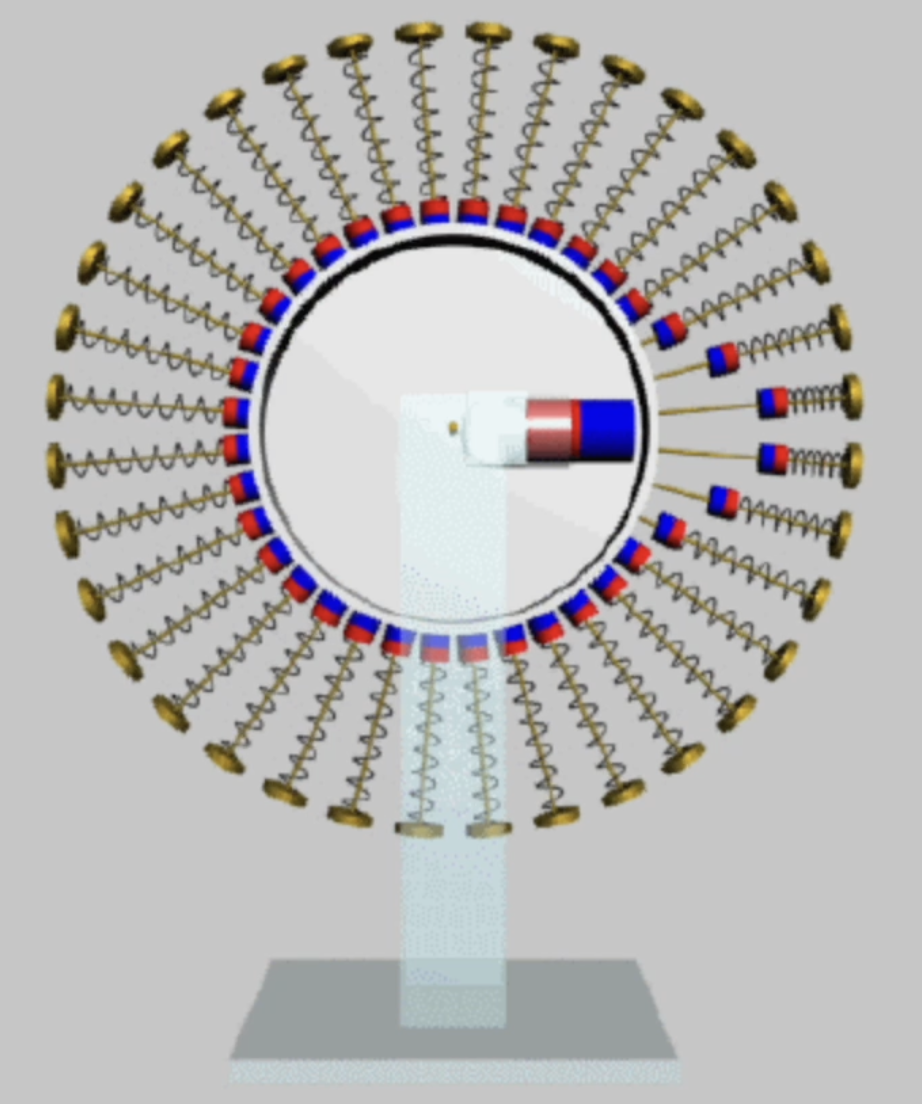
\includegraphics[width=0.2\linewidth]{2.png}
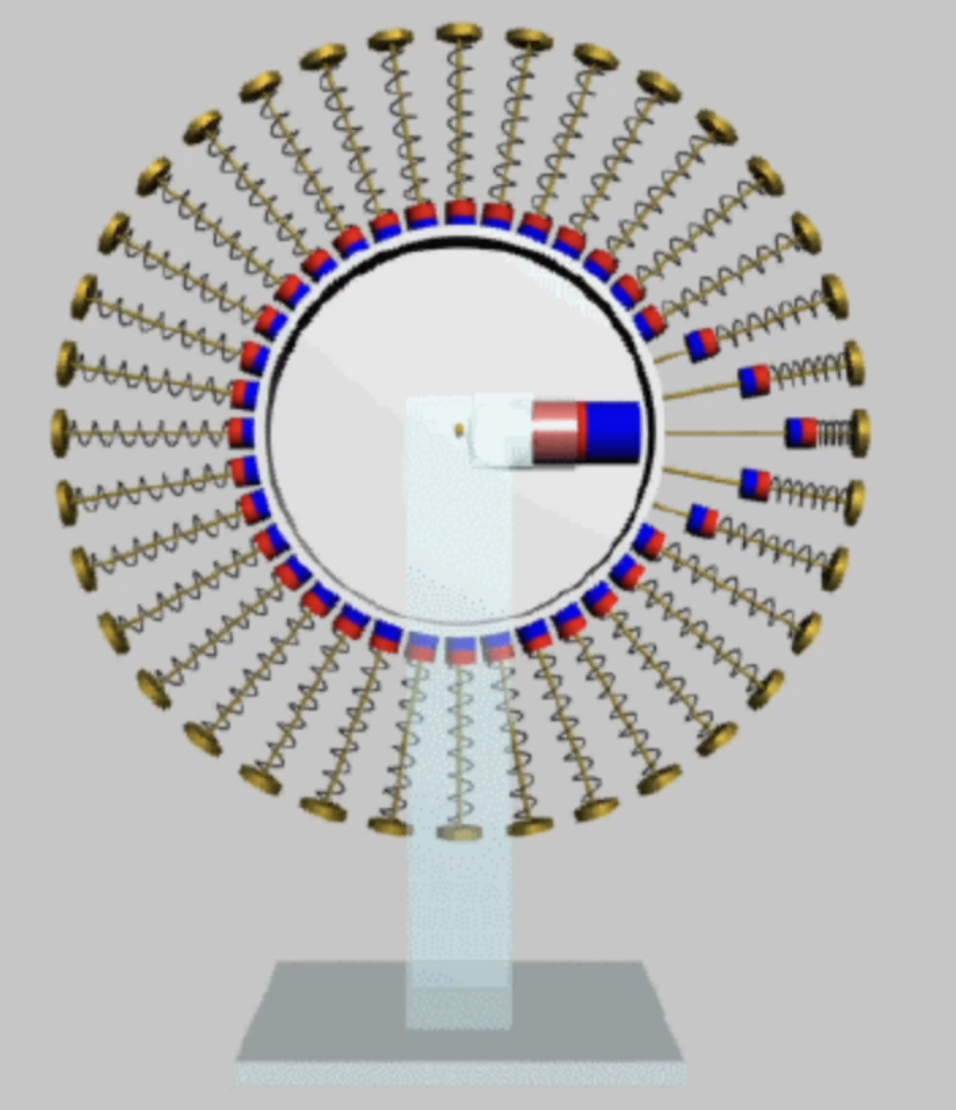
\includegraphics[width=0.2\linewidth]{3.png}
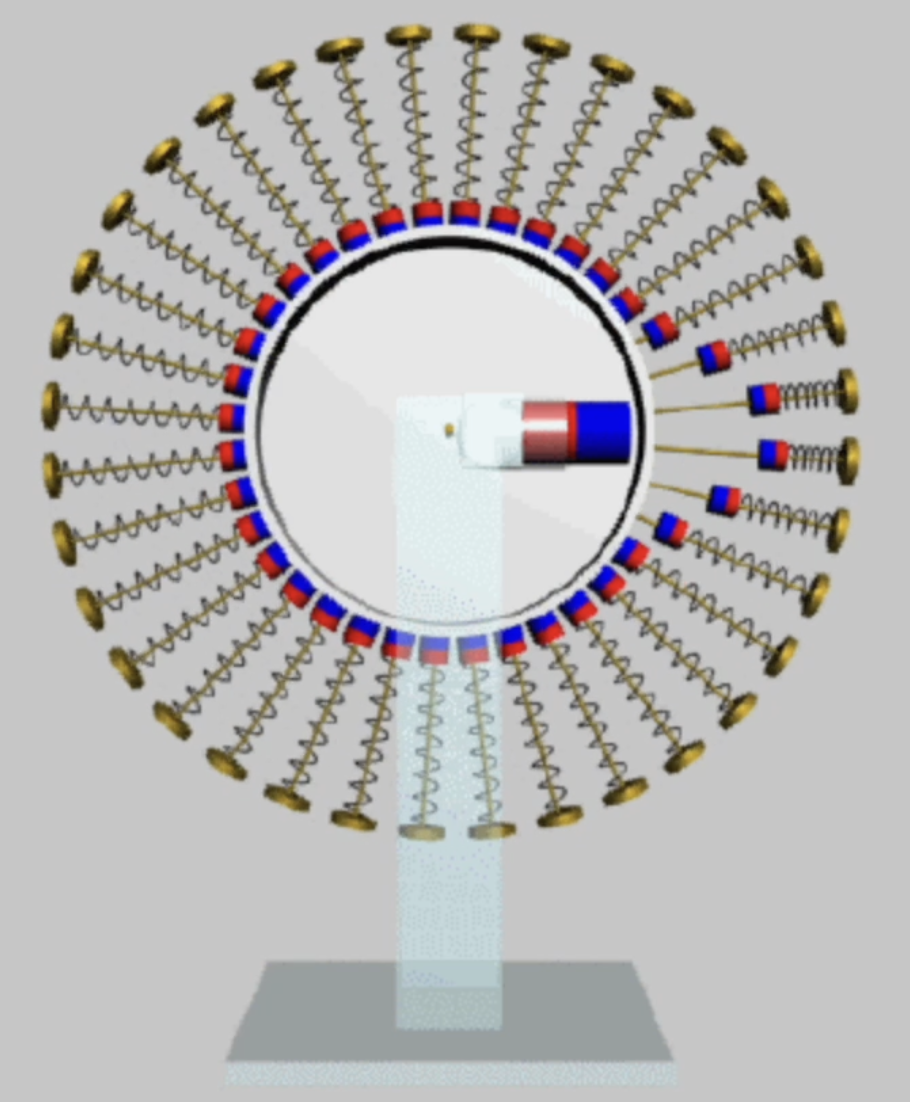
\includegraphics[width=0.2\linewidth]{4.png}
\caption{The Perpetual Motion Machine.}
\end{figure}


\section{Analysis}
\label{sec:Befor}
Now, let's analyse this quantitatively.

\subsection{Assistant model}
First, let's construct a simpler model to assist us in the analysis, as shown in the Figure 2. 
\begin{figure}[h]
    \centering
    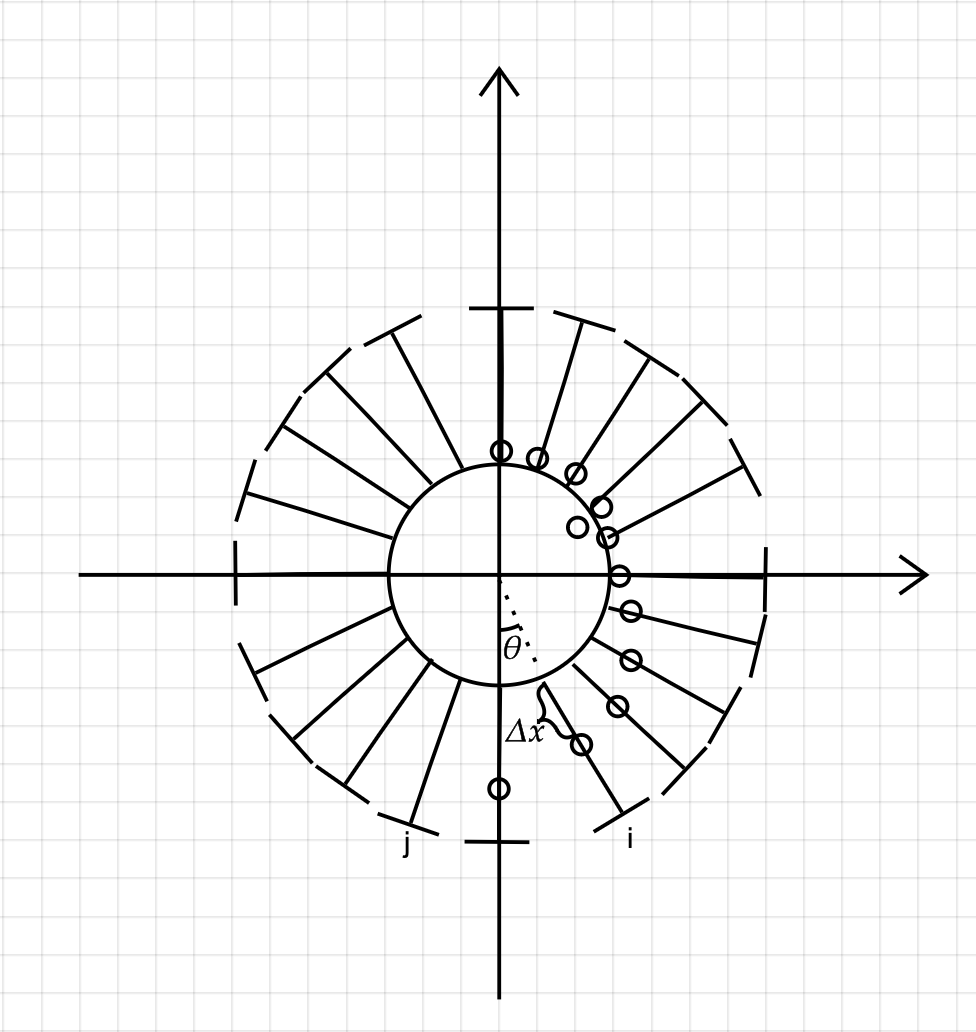
\includegraphics[width=0.5\linewidth]{5.png}
    \caption{The Simpler Model.}
\end{figure}

Suppose there is no central large magnet in the system, and each small magnet is only subject to gravitational forces. Assuming the spring has an elastic coefficient of $k$, then establish a Cartesian coordinate system. We know in this model, the system is symmetric by the y-axis. Analysing the first quadrant, we have
$$
\Delta x = 0.
$$

The compression length of the spring due to the gravitational force in the second quadrant is
$$
\Delta x = \frac{mg \cos{\theta}}{k}.
$$

The torque generated by one stick is
$$
\vec{M} = (\vec{r}+\Delta \vec{x}) \times m\vec{g}.
$$

We know the torque generated by the right part and the left part has the same magnitude, but the opposite direction, so we have the total torque is 
$$
\vec{M}_{all} = 0
$$

Without considering other disturbances such as friction, if we provide an initial angular velocity, the system will maintain equilibrium and continue to move at that angular velocity indefinitely. However, it will not be able to perform any external work.

\subsection{Real model}
Now, let's introduce the central large magnet into the system, as shown in the Figure 3.
\begin{figure}[h]
    \centering
    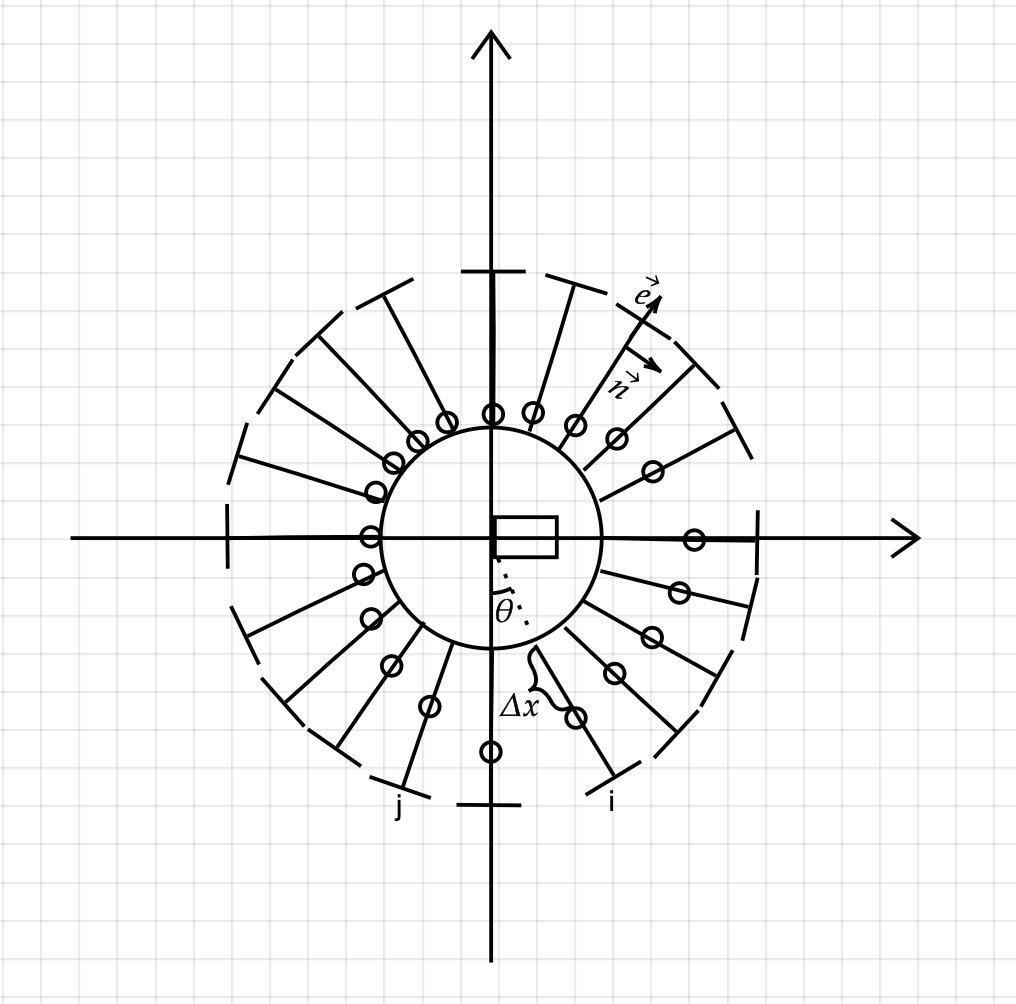
\includegraphics[width=0.5\linewidth]{6.png}
    \caption{The Real Model.}
\end{figure}

Assuming that the magnetic force experienced by our small magnet is a function distributed on the x-y plane, we have $F_{mag} = f(x, y)$. Let's assume that the magnetic force on the left side can be neglected, and we will only consider the forces on the right side. We will establish a local coordinate system on each slender rod, with the direction of the rod denoted by the unit vector $\vec{e}$ and the direction perpendicular to the rod denoted by the unit vector $\vec{n}$. We can observe that the distribution of the small magnets is not uniform in this case. In the first quadrant, the torque generated by the small magnet is given by
$$
\vec{M} = ( \vec{r}+ \frac{f_e(x,y) - mg \cos{\theta}}{k}\cdot\vec{e})\times (m\vec{g} + f_n(x,y)\cdot\vec{n}).
$$

Similarly, in the fourth quadrant, we have
$$
\vec{M} = ( \vec{r}+\frac{f_e(x,y) + mg \cos{\theta}}{k}\cdot\vec{e})\times (m\vec{g} + f_n(x,y)\cdot\vec{n}).
$$

The analysis for the left side would be the same as our initial simplified model, where we neglect the magnetic forces and consider only the gravitational forces acting on the small magnets.

If we continue the analysis based on left-right symmetry and consider only the torque generated by the force of $m\vec{g}$, we would conclude that $\vec{M}_{all}>0$ (where $M_{all}$ represents the total torque). This would lead to the conclusion that the device can perform work without the input of energy.

However, this conclusion is based on the assumption that we are neglecting the torque generated by the force $f_n(x,y)$. In reality, this force would contribute to the overall torque and cannot be ignored.

According to the analysis, it is observed that the compression of the spring in the fourth quadrant is larger than in the first quadrant. Consequently, for the corresponding positions of the small magnets, the distance in the fourth quadrant is greater than in the first quadrant. This implies that the magnitude of the force $f_n$ in the first quadrant is larger than in the fourth quadrant.

And since
$$
B = 2k\frac{M}{z^3}.
$$

So, we can derive that the decay of a magnetic field is inversely proportional to the cube of the distance, then we can get
$$
( \vec{r}+ \frac{f_e(x_1,y_1) - mg \cos{\theta}}{k}\cdot\vec{e})\times f_n(x_1,y_1)\cdot\vec{n} > ( \vec{r}+ \frac{f_e(x_4,y_4) + mg \cos{\theta}}{k}\cdot\vec{e})\times f_n(x_4,y_4)\cdot\vec{n}.
$$

Namely, We would have a torque pointing outward, but this torque would eventually be effectively cancelled out by the torque in the inward direction. In the end, we would still have $\vec{M}_{all} = 0$.

Therefore, the device would not be able to perform work on the external environment.

\subsection{Decay of Permanent Magnet's Magnetic Properties}
In addition, permanent magnets do not actually maintain a constant magnetic field indefinitely. When a magnet is exposed to other magnetic fields, demagnetization can occur. This demagnetization phenomenon is more pronounced when strong magnets are used. In this experiment, by utilizing magnetic force to push the small magnet away, and employing the measure of increasing the lever arm, the magnetic energy is effectively converted into other forms of energy. However, these energy forms do not convert back into magnetic energy. As a result, the magnet's magnetic properties will decay over time, and eventually, the device will no longer function as effectively as it did initially.

\section{Conclusion}
\label{sec:con}
The text provides a detailed quantitative analysis of the magnetic spring perpetual motion machine mentioned earlier, demonstrating that the device, in theory, cannot generate work without absorbing energy from the external environment. This proves that the magnetic spring perpetual motion machine is not feasible.

\end{document} 